\usetheme{Berlin}

\usepackage[utf8]{inputenc}
\usepackage[T1]{fontenc}
\usepackage{lmodern}
\usepackage{amsthm}
\usepackage{amsmath}
\usepackage{graphicx}
\usepackage{float}
\usepackage{caption}
\captionsetup{labelformat=empty,labelsep=none}
\DeclareMathOperator*{\E}{\mathbb{E}}

\title{Encoding funny games into SAT}
\author[N. Grosshans \& T. Rohrmann]{Nathan Grosshans and Till Rohrmann}
\institute[École Polytechnique]{École Polytechnique}
\date{\today}
\subject{Encoding funny games into SAT}


\begin{document}
		\frame{\titlepage}
		\begin{frame}
			\frametitle{Table of Contents}
			\tableofcontents
		\end{frame}
		\section{Introduction}

\begin{frame}
	\frametitle{Problem description}
	\begin{columns}
		\begin{column}{5cm}
			\begin{itemize}
				\item<1-> Problem: Solving a game
				\item<2-> Means: Reduction to SAT
				\item<3-> SAT well understood and efficient solvers
			\end{itemize}
			
		\end{column}
		\begin{column}{6cm}
			\begin{figure}
				\centering
				
\includegraphics[width=5.5cm]{images/gameover.png}
			\end{figure}
		\end{column}
	\end{columns}
	\begin{block}{Goal}<4->
				Show expressiveness of propositional logic and applicability of SAT reduction for complex problems
	\end{block}
	
\end{frame}



		\section{Skyscraper}

\begin{frame}
	\frametitle{Skyscraper}
	\begin{block}{Description}<1->
		\begin{itemize}
			\item Quadratic field with side length $n$
			\item Place differently sized skyscraper on field, height $\in[1,n]$
		\end{itemize}
	\end{block}
	\begin{block}{Constraints}<2->
		\begin{itemize}
			\item No two skyscraper on one field
			\item No two skyscraper with the same height in each row/column
			\item Number of visible skyscrapers seen from the side
		\end{itemize}
	\end{block}
\end{frame}

\begin{frame}
	\frametitle{Example}
	\begin{figure}
		\centering
		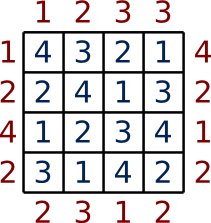
\includegraphics[height=6cm]{images/skyscraper.png}
	\end{figure}
\end{frame}

\begin{frame}
	\frametitle{Encoding}
	\begin{block}{State space}<1->
		\begin{itemize}
			\item Skyscraper variables: $v_{x,y}^{h}$ with $x,y,h\in[1,n]$
			\item Semantic: $v_{x,y}^{h} \equiv 1 \Leftrightarrow$ Skyscraper with height $h$ on field $x,y$
		\end{itemize}
	\end{block}
	\begin{itemize}
		\item<2-> On every field there has to be at least one skyscraper
		\begin{displaymath}
			\bigwedge_{x,y} \left( \bigvee_{h} v_{x,y}^h\right)
		\end{displaymath}
	\end{itemize}
\end{frame}

\begin{frame}
	\frametitle{Encoding cont.}
	\begin{itemize}
		\item On every field there has to be at most one skyscraper
		\begin{displaymath}
			\bigwedge_{x,y} \bigwedge_{h\not=h^{\prime}} \neg(v_{x,y}^{h} \wedge v_{x,y}^{h^{\prime}})
		\end{displaymath}
		\item<2-> No two equally high skyscraper in each row/column
		\begin{displaymath}
			\bigwedge_{h,c} \bigwedge_{k\not=l} \neg(v_{c,k}^{h} \wedge v_{c,l}^{h}) \wedge \neg (v_{k,c}^{h} \wedge v_{l,c}^{h})
		\end{displaymath}
	\end{itemize}
\end{frame}

\begin{frame}
	\frametitle{Constraint encoding}
	\begin{itemize}
		\item Counting function $numS$ and memory function $maxS$
		\begin{displaymath}
			maxS_{d}(\pmb x) = 
			\begin{cases}
				height(\pmb x) & height(\pmb x) > maxS_{d}(\pmb x + \pmb e_{d})\\
				maxS_{d}(\pmb x + \pmb e_{d}) &\text{if not}
			\end{cases}
		\end{displaymath}
		\begin{displaymath}
			numS_{d}(\pmb x) =
			\begin{cases}
				numS_{d}(\pmb x + \pmb e_{d}) + 1 & height(\pmb x) > maxS_{d}(\pmb x + \pmb e_{d})\\
				numS_{d}(\pmb x + \pmb e_{d}) &\text{if not}
			\end{cases}
		\end{displaymath}
		\item $d\in \{North, East, South, West\}$
		\item $\pmb e_{North} = (-1,0)^T, \pmb e_{East} = (0,1)^T, \pmb e_{South} = (1,0)^T,\pmb e_{West} = (0,-1)^T$
	\end{itemize}
\end{frame}

\begin{frame}
	\frametitle{Constraint encoding cont.}
	\begin{columns}
		\begin{column}{6cm}
			\begin{itemize}
				\item Constraint $c$ adds clause $numS_{d}(\pmb x) = c$ to formula
				\item <2-> Polynomial reduction in side length of field $O(n^3)$
			\end{itemize}
		\end{column}
		\begin{column}{5cm}<2->
			\begin{figure}
				\centering
				
\includegraphics[width=5cm]{images/win.jpg}
			\end{figure}
		\end{column}
	\end{columns}
\end{frame}

\begin{frame}
	\centering
	\hfill \Large Live demonstration \hfill\hfill
\end{frame}

		\section{Hex-a-Hop}

\begin{frame}
	\frametitle{Hex-a-Hop}
	\begin{columns}
		\begin{column}{6cm}
			\begin{itemize}
				\item Hexagonal puzzle game
				\item<2-> Goal: Destroy all green tiles by walking on them
				\item<3-> Special tiles: Trampolines, turquoise tiles, high tiles
				\item<4-> Dynamic behavior depends on player's moves
			\end{itemize}
		\end{column}
		\begin{column}{5cm}
			\begin{figure}
				\centering
				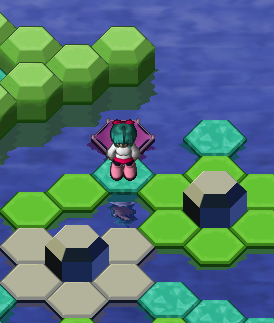
\includegraphics[width=5cm]{images/hexahop.png}
			\end{figure}
		\end{column}
	\end{columns}
\end{frame}

\begin{frame}
	\frametitle{Encoding}
	\begin{block}{State space}
		\begin{itemize}	
			\item Boolean variables $v_{x,y}^{t}$ with $(x,y)$ position on field, $t$ time step
			\item Semantic: $v_{x,y}^{t} \equiv 1 \Leftrightarrow$ Player is at time step $t$ at position $(x,y)$
		\end{itemize}
	\end{block}

	\pause

	\begin{itemize}
		\item At each time step, the player has to be somewhere
			  \begin{displaymath}
			  \bigwedge \limits_t (\bigvee \limits_{x, y} v_{x,y}^{t})
			  \end{displaymath}
		\pause
		\item But the player can't be at two positions at the same time
			  \begin{displaymath}
			  \bigwedge \limits_{\substack{t\\ {(x, y) \not= (x', y')}}}
			  (\neg v_{x,y}^{t} \vee \neg v_{x',y'}^{t})
			  \end{displaymath}
	\end{itemize}
\end{frame}

\begin{frame}
	\frametitle{Movement behavior}
	\begin{columns}
		\begin{column}{6cm}
			\begin{itemize}
				\item How to encode legal moves?
				\item<2-> $\forall x,y:$ calculate set of neighbors $N$
				\begin{displaymath}
					\bigwedge_{x,y,t} v_{x,y}^t \Rightarrow \bigvee_{n\in N} v_{n}^{t+1}
				\end{displaymath}
			\end{itemize}
		\end{column}
		\begin{column}{5cm}
			\begin{figure}
				\centering
				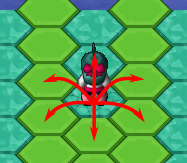
\includegraphics[width=5cm]{images/movement.png}
			\end{figure}
		\end{column}
	\end{columns}
\end{frame}

\begin{frame}
	\frametitle{Dynamic tiles}
	\begin{itemize}
		\item Tile behavior when visited
		\begin{displaymath}
			\text{Turquoise} \Rightarrow \text{Green} \Rightarrow \text{Destroyed}
		\end{displaymath}
		\pause
		\item Dynamic type function
		\begin{displaymath}
			dT(\pmb x,t+1)=
			\begin{cases}
				dT(\pmb x, t) & v_{\pmb x}^{t} \not \equiv 1\\
				\text{Destroyed} & v_{\pmb x}^{t} \equiv 1 \wedge dT(\pmb x,t) = \text{Green}\\
				\text{Green} & v_{\pmb x}^{t} \equiv 1 \wedge dT(\pmb x,t)=\text{Turquoise}
			\end{cases}
		\end{displaymath}
		\pause
		\item Allows to define behavioral clauses easily
	\end{itemize}
\end{frame}

\begin{frame}
	\frametitle{Start \& end condition}
	\begin{block}{Start condition}
		\begin{itemize}
			\item Add start position $\pmb x$ to clauses: $v_{\pmb x}^{0}$
		\end{itemize}
	\end{block}

	\begin{block}{End condition}
		\begin{itemize}
			\item All green tiles have to be destroyed
			\begin{displaymath}
				\bigwedge_{\pmb x} \neg (dT(\pmb x, t_{max}) = \text{Green})
			\end{displaymath}
			\item $t_{max}$ last timestep
		\end{itemize}
	\end{block}
\end{frame}

\begin{frame}
	\frametitle{Advanced tile types}
	\begin{block}{Trampolines}
		\begin{itemize}
			\item Accessibility thanks to a sequel of jumps
			\pause
			\item Variable $trampoline_t$ indicating whether or not we used
				  a trampoline at time step $t$
		\end{itemize}
	\end{block}

	\pause

	\begin{block}{High tiles}
		\begin{itemize}
			\item Variables $h_{green}^t$ and $h_{turquoise}^t$ indicating
				  whether the high tiles of a given type have sunk down
			\pause
			\item Accessibility at time step $t$ depending on those
				  variables
			\pause
			\item Special case to consider for trampolines
		\end{itemize}
	\end{block}
\end{frame}

\begin{frame}
	\centering
	\hfill \Large Live demonstration \hfill\hfill
\end{frame}

		\section{Conclusion}

\begin{frame}
	\frametitle{Conlusion}
	\begin{columns}
		\begin{column}{6cm}
			\begin{itemize}
				\item Successfully solved Skyscraper and parts of Hex-a-Hop
				\item<2-> Express complex dynamics with propositional logic
				\item<3-> Use existing SAT solver to solve SAT problem
				\item<4-> However: Quick increase of formula size with increasing complexity
			\end{itemize}
		\end{column}
		\begin{column}{5cm}
			\centering
			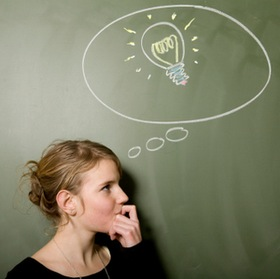
\includegraphics[width=4.5cm]{images/bulb.jpg}
		\end{column}
	\end{columns}

\end{frame}

\end{document}
